\documentclass[aspectratio=169, table]{beamer}

\usepackage{colortbl}
\usepackage{xcolor}
\usepackage{listings}
\usepackage{pgfplots}
\usepgfplotslibrary{polar}
\usepackage{tikz}
\usetikzlibrary{shapes.geometric,
	positioning, shapes, shapes.multipart, backgrounds, arrows.meta, calc, fit, trees}

\usetheme{Pradita}

\lstdefinelanguage{xml}{
	keywords={},
	basicstyle=\ttfamily\scriptsize,
	keywordstyle=\color{blue}\bfseries,
	sensitive=true,
	commentstyle=\color{gray}\ttfamily,
	stringstyle=\color{purple}\ttfamily,
	numbers=left,
	numberstyle=\tiny\color{gray},
	breaklines=true,
	frame=lines,
	backgroundcolor=\color{lightgray!10},
	tabsize=2,
	morecomment=[s]{<!--}{-->},
	morestring=[b]",
	morestring=[b]',
	showstringspaces=false
}

\lstdefinelanguage{emfatic}{
  keywords={package,enum,class,abstract,attr,ref,val,extends},
  keywordstyle=\color{blue}\bfseries,
  sensitive=true,
  comment=[l]{//},
  commentstyle=\color{gray}\ttfamily,
  basicstyle=\ttfamily\scriptsize,
  numbers=left,
  numberstyle=\tiny\color{gray},
  breaklines=true,
  frame=lines,
  backgroundcolor=\color{lightgray!10},
  showstringspaces=false
}

\lstdefinelanguage{java}{
  keywords={package,import,public,class,interface,extends,implements,
            return,new,null,true,false,void,if,else,for,while,static,
            final,private,protected,override,Override},
  keywordstyle=\color{blue}\bfseries,
  sensitive=true,
  comment=[l]{//},
  morecomment=[s]{/*}{*/},
  commentstyle=\color{gray}\ttfamily\itshape,
  stringstyle=\color{purple}\ttfamily,
  morestring=[b]",
  basicstyle=\ttfamily\scriptsize,
  numbers=left,
  numberstyle=\tiny\color{gray},
  breaklines=true,
  frame=lines,
  backgroundcolor=\color{lightgray!10},
  showstringspaces=false
}

\subtitle{IT30213 - Advanced Software Engineering \& DevOps}
\title{\Huge Visual Domain-Specific\vspace{8pt}\\
	Language}
\author{\textbf{Alfa Yohannis}}

\begin{document}

\frame{\titlepage}

\begin{frame}[fragile]
	\frametitle{Contents}
	\vspace{20pt}
	\begin{columns}[t]
		\column{0.5\textwidth}
		\tableofcontents[sections={1-6}]

		\column{0.5\textwidth}
		\tableofcontents[sections={7-14}]
	\end{columns}
\end{frame}

\begin{frame}{\hfill}
	\centering
	\Huge{\textbf{Bagaimana jika pipeline media bisa\\[8pt]
	didesain hanya dengan drag-and-drop?}}
\end{frame}

% ============================================================
\section{Tujuan Pembelajaran}
\begin{frame}{\hfill}
	\centering
	\Huge{\textbf{Tujuan Pembelajaran}}
\end{frame}

\begin{frame}{Tujuan Pembelajaran}
\vspace{6pt}
Setelah sesi ini, mahasiswa diharapkan mampu:
\begin{enumerate}
  \item Menjelaskan perbedaan pendekatan \textit{visual DSL} dibandingkan \textit{textual DSL} dan alasan penggunaan notasi grafis sebagai representasi model domain.
  \item Menerapkan metodologi pengembangan visual DSL menggunakan Eclipse Sirius: perancangan viewpoint, mapping grafis, konfigurasi palet, dan pembuatan model instans.
  \item Menganalisis trade-off antara visual DSL dan textual DSL serta menentukan pendekatan yang paling sesuai untuk konteks tim dan pengguna.
\end{enumerate}
\end{frame}

% ============================================================
\section{Pendahuluan}
\begin{frame}{\hfill}
	\centering
	\Huge{\textbf{Pendahuluan}}
\end{frame}

\begin{frame}{Textual DSL: Kuat, tetapi Ada Batasnya}
\vspace{6pt}
\begin{columns}[T]
\column{0.5\textwidth}
\textbf{Kelebihan Textual DSL}
\begin{itemize}
  \item Mudah diversi di Git.
  \item Dapat dibuat secara programatik.
  \item Kompak dan ringkas.
  \item Ramah CI/CD pipeline.
\end{itemize}

\column{0.5\textwidth}
\textbf{Keterbatasan}
\begin{itemize}
  \item Barrier masuk: perlu belajar sintaks.
  \item Topologi bercabang sulit dibayangkan dari teks.
  \item Kesalahan koneksi port tidak terdeteksi visual.
  \item Kolaborasi non-developer terhambat.
\end{itemize}
\end{columns}

\vspace{12pt}
\small
\textit{Visual DSL} hadir sebagai pendekatan komplementer: model dinyatakan dalam notasi grafis, bukan teks, tetapi tetap disimpan sebagai XMI yang dapat diversi dan divalidasi.
\end{frame}

\begin{frame}{Drag-and-Drop, Model Tetap Tersimpan}
\vspace{6pt}
\begin{columns}[T]
\column{0.5\textwidth}
\textbf{Cara Kerja Visual DSL}
\begin{itemize}
  \item Pengguna menggambar diagram di kanvas.
  \item Node dibuat via palet, port dihubungkan dengan panah.
  \item Model XMI dihasilkan/diperbarui otomatis di balik layar.
  \item Diagram dan model selalu sinkron.
\end{itemize}

\column{0.5\textwidth}
\textbf{Fondasi Tetap Sama}
\begin{itemize}
  \item Metamodel \texttt{mediaflow.ecore} tidak berubah.
  \item Visual DSL hanya menambahkan \textit{lapisan presentasi} di atas metamodel yang sudah ada.
  \item Model XMI hasil visual DSL kompatibel dengan tooling EMF lainnya.
\end{itemize}
\end{columns}
\end{frame}

% ============================================================
\section{Masalah Domain}
\begin{frame}{\hfill}
	\centering
	\Huge{\textbf{Masalah Domain}}
\end{frame}

\begin{frame}{Masalah Utama yang Mendorong Visual DSL}
\vspace{6pt}
\begin{enumerate}
  \item \textbf{Pemahaman topologi terbatas.} Pengguna non-teknis sulit membayangkan alur percabangan dari teks DSL.
  \item \textbf{Kesalahan referensi port sulit dideteksi.} Koneksi keliru antara port \texttt{OUT} dan \texttt{IN} tidak terlihat dalam teks.
  \item \textbf{Barrier masuk tinggi.} Perlu memahami sintaks DSL sebelum bisa mulai memodelkan.
  \item \textbf{Kolaborasi desainer-developer sulit.} Arsitek dan operator tidak menggunakan tool yang sama.
  \item \textbf{Navigasi model kompleks lambat.} Menelusuri relasi antar-komponen di teks lebih lambat daripada di diagram.
\end{enumerate}
\end{frame}

\begin{frame}{Kebutuhan Pemodelan Visual}
\vspace{6pt}
\begin{enumerate}
  \item \textbf{Notasi grafis berbasis domain} --- membedakan \texttt{Resource}, \texttt{Scaler}, \texttt{Transcoder} via warna dan bentuk.
  \item \textbf{Port sebagai titik koneksi grafis} --- dihubungkan drag-and-drop membentuk \texttt{Edge}.
  \item \textbf{Label informatif dari model} --- nilai atribut kunci tampil langsung di diagram.
  \item \textbf{Palet alat untuk pembuatan elemen} --- tanpa menulis teks.
  \item \textbf{Konsistensi model-diagram otomatis} --- perubahan diagram $\leftrightarrow$ model XMI langsung sinkron.
  \item \textbf{Reuse metamodel yang sudah ada} --- notasi visual ditambahkan, kontrak domain tidak diulang.
\end{enumerate}
\end{frame}

% ============================================================
\section{Metodologi}
\begin{frame}{\hfill}
	\centering
	\Huge{\textbf{Metodologi Pengembangan Visual DSL}}
\end{frame}

\begin{frame}{7 Langkah Metodologi Visual DSL}
\vspace{4pt}
\begin{columns}[T]
\column{0.5\textwidth}
\begin{enumerate}
  \item \textbf{Penetapan metamodel} sebagai fondasi bersama.
  \item \textbf{Pemilihan framework} visual DSL (Sirius, GMF, GLSP).
  \item \textbf{Perancangan notasi grafis}: bentuk, warna, label, ikon.
  \item \textbf{Definisi viewpoint specification} (\texttt{.odesign}).
\end{enumerate}

\column{0.5\textwidth}
\begin{enumerate}
  \setcounter{enumi}{4}
  \item \textbf{Pembuatan model instans} melalui diagram editor.
  \item \textbf{Validasi dan eksplorasi} model secara grafis.
  \item \textbf{Integrasi dan pengujian} tooling berbasis EMF.
\end{enumerate}
\end{columns}

\vspace{10pt}
\small
\textbf{Prinsip kunci:} notasi visual hanya \textit{mempresentasikan} elemen metamodel, bukan mendefinisikannya ulang. Perubahan semantik domain harus dilakukan di metamodel, bukan di \texttt{.odesign}.
\end{frame}

\begin{frame}{Notasi Visual untuk MediaFlow}
\vspace{6pt}
\centering
\footnotesize
\begin{tabular}{|l|l|l|l|}
\hline
\rowcolor{blue!12}
\textbf{Elemen} & \textbf{Bentuk} & \textbf{Warna} & \textbf{Label (AQL)} \\
\hline
\texttt{Resource} & Container (persegi) & Biru muda & \texttt{name [mediaType]} \\
\hline
\texttt{Scaler} & Ellipse & Hijau muda & \texttt{name (width x height)} \\
\hline
\texttt{Transcoder} & Ellipse & Oranye muda & \texttt{name [videoCodec/audioCodec]} \\
\hline
\texttt{Port} & Bordered node (kotak kecil) & Sesuai induk & \texttt{name} \\
\hline
\texttt{Edge} & Panah ($\rightarrow$) & Hitam & \texttt{name} \\
\hline
\end{tabular}

\vspace{10pt}
\small
AQL (\textit{Acceleo Query Language}) digunakan untuk ekspresi label dinamis yang langsung diturunkan dari atribut model.
\end{frame}

% ============================================================
\section{Arsitektur Sirius}
\begin{frame}{\hfill}
	\centering
	\Huge{\textbf{Arsitektur Eclipse Sirius}}
\end{frame}

\begin{frame}{Dua Proyek Utama}
\vspace{4pt}
\begin{columns}[T]
\column{0.5\textwidth}
\textbf{Proyek \texttt{mediaflow} (Metamodel)}
\begin{itemize}
  \item \texttt{metamodels/mediaflow.ecore}
  \item \texttt{metamodels/mediaflow.genmodel}
  \item \texttt{src/mediaflow/...} (kelas Java EMF)
\end{itemize}

\vspace{8pt}
\textbf{Alur Data}
\begin{center}
\scalebox{0.8}{
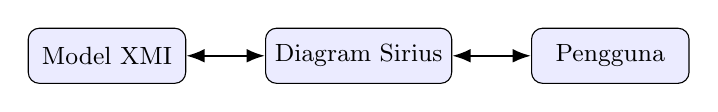
\begin{tikzpicture}[>=Latex, node distance=10mm, box/.style={draw,rounded corners,minimum width=2cm,minimum height=0.7cm,align=center,fill=blue!8,font=\small}]
  \node[box] (xmi) {Model XMI};
  \node[box, right=of xmi] (sirius) {Diagram Sirius};
  \node[box, right=of sirius] (user) {Pengguna};
  \draw[<->, thick] (xmi) -- (sirius);
  \draw[<->, thick] (sirius) -- (user);
\end{tikzpicture}
}
\end{center}

\column{0.5\textwidth}
\textbf{Proyek \texttt{mediaflow.sirius} (Visual DSL)}
\begin{itemize}
  \item \texttt{description/mediaflow.odesign}
  \item \texttt{icons/} (resource, scaler, transcoder, port, edge)
  \item \texttt{src/mediaflow/sirius/ Services.java}
  \item \texttt{flow1.mediaflow}, \texttt{flow2.mediaflow}
  \item \texttt{representations.aird}
\end{itemize}
\end{columns}
\end{frame}

% ============================================================
\section{Implementasi: Viewpoint \& Mappings}
\begin{frame}{\hfill}
	\centering
	\Huge{\textbf{Implementasi: Viewpoint \& Mappings}}
\end{frame}

\begin{frame}[fragile]{Viewpoint dan Diagram Description}
\vspace{6pt}
\begin{lstlisting}[language=xml, basicstyle=\ttfamily\scriptsize]
<description:Group name="mediaflow">
  <ownedViewpoints name="graph"
      modelFileExtension="mediaflow">
    <ownedRepresentations
        xsi:type="description_1:DiagramDescription"
        name="MediaFlow diagram"
        domainClass="mediaflow::Graph"
        synchronized="true"
        showOnStartup="true">
      <metamodel href="mediaflow#/"/>
      <defaultLayer name="Default">
        <!-- mappings dan tools di sini -->
      </defaultLayer>
    </ownedRepresentations>
  </ownedViewpoints>
</description:Group>
\end{lstlisting}
\vspace{2pt}
\small \texttt{domainClass="mediaflow::Graph"} mengikat diagram ke kelas root metamodel.\\
\texttt{synchronized="true"} menjaga konsistensi diagram--model XMI secara otomatis.
\end{frame}

\begin{frame}[fragile]{Resource: Container \& Bordered Node Port}
\vspace{4pt}
\begin{columns}[T]
\column{0.55\textwidth}
\begin{lstlisting}[language=xml, basicstyle=\ttfamily\tiny]
<containerMappings name="ResourceContainer"
    semanticCandidatesExpression="feature:nodes"
    domainClass="mediaflow::Resource">
  <borderedNodeMappings name="PortInResource"
      semanticCandidatesExpression="feature:ports"
      domainClass="mediaflow::Port">
    <style xsi:type="style:SquareDescription"
        labelExpression="aql:self.name"
        width="2" height="2">
      <color href="environment:/...dark_blue"/>
    </style>
  </borderedNodeMappings>
  <style xsi:type="style:FlatContainerStyleDescription"
      labelExpression="aql:self.name
        + ' [' + self.mediaType.toString() + ']'"
      roundedCorner="true">
    <backgroundColor href="environment:/...light_blue"/>
  </style>
</containerMappings>
\end{lstlisting}

\column{0.45\textwidth}
\vspace{10pt}
\textbf{Poin kunci}
\begin{itemize}
  \item \texttt{feature:nodes} --- kandidat semua node bertipe \texttt{Resource}.
  \item \texttt{feature:ports} --- port ditampilkan sebagai bordered node di tepi container.
  \item Label AQL: \texttt{name [VIDEO]} diturunkan dari atribut model.
  \item Warna: biru muda (\texttt{light\_blue}).
\end{itemize}
\end{columns}
\end{frame}

\begin{frame}[fragile]{Scaler dan Transcoder: Ellipse Node}
\vspace{4pt}
\begin{columns}[T]
\column{0.52\textwidth}
\begin{lstlisting}[language=xml, basicstyle=\ttfamily\tiny]
<!-- Scaler: ellipse hijau -->
<nodeMappings name="ScalerNode"
    semanticCandidatesExpression="feature:nodes"
    domainClass="mediaflow::Scaler">
  <borderedNodeMappings name="PortInScaler"
      semanticCandidatesExpression="feature:ports"
      domainClass="mediaflow::Port">
    ...
  </borderedNodeMappings>
  <style xsi:type="style:EllipseNodeDescription"
      iconPath="/icons/scaler.png"
      labelExpression="aql:self.name
        + ' (' + self.width + 'x' + self.height + ')'">
    <color href="environment:/...light_green"/>
  </style>
</nodeMappings>

<!-- Transcoder: ellipse oranye -->
<nodeMappings name="TranscoderNode" ...
    domainClass="mediaflow::Transcoder">
  <style xsi:type="style:EllipseNodeDescription"
      labelExpression="aql:self.name
        + ' [' + self.videoCodec
        + '/' + self.audioCodec + ']'">
    <color href="environment:/...light_orange"/>
  </style>
</nodeMappings>
\end{lstlisting}

\column{0.48\textwidth}
\vspace{10pt}
\textbf{Label AQL per jenis node}
\begin{itemize}
  \item \texttt{Scaler}: \texttt{scaler\_1080 (1920x1080)}
  \item \texttt{Transcoder}: \texttt{transcoder\_h264 [h264/aac]}
\end{itemize}

\vspace{8pt}
\textbf{Label selalu sinkron}\\
Nilai label diturunkan langsung dari atribut model --- berubah di model, langsung update di diagram.
\end{columns}
\end{frame}

\begin{frame}[fragile]{Edge Mapping: Koneksi Antar Port}
\vspace{6pt}
\begin{lstlisting}[language=xml, basicstyle=\ttfamily\scriptsize]
<edgeMappings name="EdgeMapping"
    semanticCandidatesExpression="feature:edges"
    domainClass="mediaflow::Edge"
    useDomainElement="true"
    sourceFinderExpression="feature:source"
    targetFinderExpression="feature:target"
    sourceMapping="...PortInResource ...PortInScaler ...PortInTranscoder"
    targetMapping="...PortInResource ...PortInScaler ...PortInTranscoder">
  <style targetArrow="InputFillClosedArrow">
    <centerLabelStyleDescription
        labelExpression="feature:name" labelSize="9"/>
  </style>
</edgeMappings>
\end{lstlisting}
\vspace{4pt}
\small
\texttt{sourceFinderExpression="feature:source"} mengambil referensi port dari model XMI, lalu menggambarnya sebagai panah antar bordered node secara otomatis.
\end{frame}

% ============================================================
\section{Implementasi: Palette Tools}
\begin{frame}{\hfill}
	\centering
	\Huge{\textbf{Implementasi: Palette Tools}}
\end{frame}

\begin{frame}[fragile]{Tool: Membuat Scaler dari Palet}
\vspace{10pt}
\begin{columns}[T]
\column{0.58\textwidth}
\begin{lstlisting}[language=xml, basicstyle=\ttfamily\tiny]
<ownedTools xsi:type="tool:NodeCreationDescription"
    name="Scaler"
    iconPath="/icons/scaler.png"
    nodeMappings="...ScalerNode"
    forceRefresh="true">
  <initialOperation>
    <firstModelOperations
        xsi:type="tool_1:ChangeContext"
        browseExpression="var:container">
      <subModelOperations
          xsi:type="tool_1:CreateInstance"
          typeName="mediaflow::Scaler"
          referenceName="nodes">
        <subModelOperations xsi:type="tool_1:SetValue"
            featureName="name"
            valueExpression="aql:'newScaler'"/>
        <subModelOperations xsi:type="tool_1:SetValue"
            featureName="width"
            valueExpression="aql:1920"/>
        <subModelOperations xsi:type="tool_1:SetValue"
            featureName="height"
            valueExpression="aql:1080"/>
      </subModelOperations>
    </firstModelOperations>
  </initialOperation>
</ownedTools>
\end{lstlisting}

\column{0.42\textwidth}
\vspace{10pt}
\textbf{Yang terjadi saat klik Scaler di palet:}
\begin{enumerate}
  \item \texttt{CreateInstance} membuat \texttt{mediaflow::Scaler} baru.
  \item Ditambahkan ke koleksi \texttt{nodes} pada \texttt{Graph}.
  \item Nilai default diisi: \texttt{name}, \texttt{width}, \texttt{height}.
  \item Diagram langsung menampilkan ellipse hijau baru.
\end{enumerate}
\end{columns}
\end{frame}

\begin{frame}[fragile]{Tool: Membuat Edge dari Palet}
\vspace{4pt}
\begin{columns}[T]
\column{0.58\textwidth}
\begin{lstlisting}[language=xml, basicstyle=\ttfamily\tiny]
<ownedTools xsi:type="tool:EdgeCreationDescription"
    name="Edge" iconPath="/icons/edge.png" edgeMappings="...EdgeMapping" forceRefresh="true">
  <sourceVariable name="source"/>
  <targetVariable name="target"/>
  <initialOperation>
    <firstModelOperations
        xsi:type="tool_1:ChangeContext" browseExpression="aql:source.eContainer().eContainer()">
      <subModelOperations xsi:type="tool_1:CreateInstance" typeName="mediaflow::Edge" referenceName="edges">
        <subModelOperations xsi:type="tool_1:SetValue" featureName="name"
            valueExpression="aql:'edge_'+source.name+'_to_'+target.name"/>
        <subModelOperations xsi:type="tool_1:SetValue"
            featureName="source"
            valueExpression="var:source"/>
        <subModelOperations xsi:type="tool_1:SetValue"
            featureName="target"
            valueExpression="var:target"/>
      </subModelOperations>
    </firstModelOperations>
  </initialOperation>
</ownedTools>
\end{lstlisting}

\column{0.42\textwidth}
\vspace{10pt}
\textbf{Yang terjadi saat drag port ke port:}
\begin{enumerate}
  \item \texttt{source.eContainer().eContainer()} menavigasi ke \texttt{Graph} induk (Port $\subset$ Node $\subset$ Graph).
  \item \texttt{CreateInstance} membuat \texttt{mediaflow::Edge}.
  \item Nama edge di-generate otomatis dari nama port.
  \item Referensi \texttt{source} dan \texttt{target} diisi ke objek Port.
\end{enumerate}
\end{columns}
\end{frame}

% ============================================================
\section{Model Instans: flow1 dan flow2}
\begin{frame}{\hfill}
	\centering
	\Huge{\textbf{Model Instans: flow1 \& flow2}}
\end{frame}

\begin{frame}{Diagram \texttt{flow1}: Pipeline Linear (Sirius)}
\vspace{4pt}
\centering
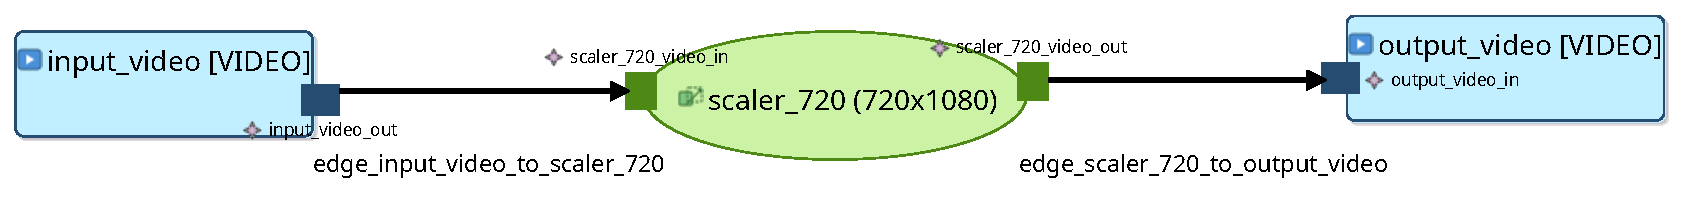
\includegraphics[width=\textwidth]{../../figures/flow1_diagram.pdf}

\vspace{4pt}
\small
\texttt{flow1.mediaflow}: Resource input $\rightarrow$ Scaler $\rightarrow$ Resource output.\\
Diagram dihasilkan oleh Eclipse Sirius dari model XMI melalui \texttt{mediaflow.odesign}.
\end{frame}

\begin{frame}{Diagram \texttt{flow2}: Pipeline Bercabang (Sirius)}
\vspace{13pt}
\centering
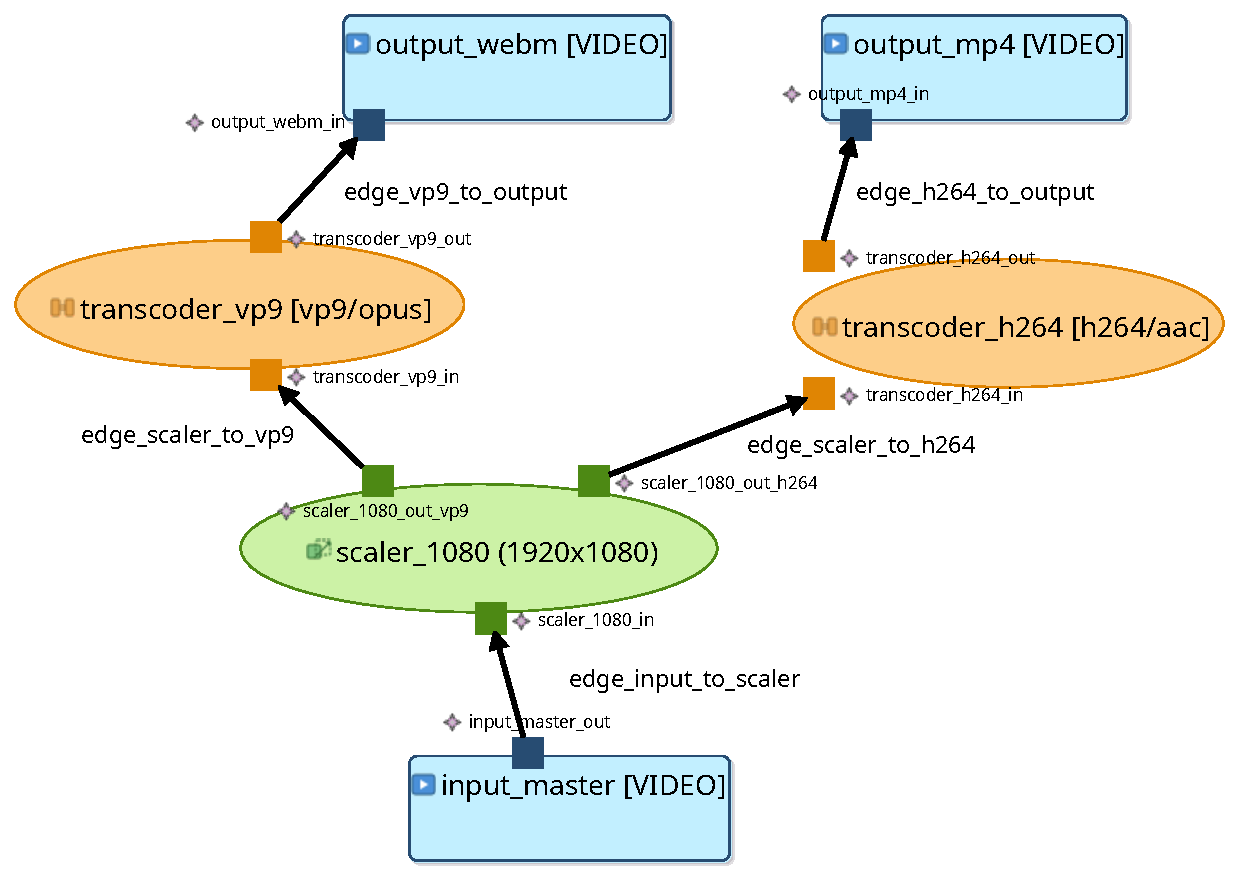
\includegraphics[width=0.6\textwidth]{../../figures/flow2_diagram.pdf}

\vspace{4pt}
\small
\texttt{flow2.mediaflow}: Resource input $\rightarrow$ Scaler $\rightarrow$ dua Transcoder $\rightarrow$ dua Resource output.\\
Topologi bercabang langsung terlihat dari diagram tanpa perlu membaca teks XMI.
\end{frame}

\begin{frame}[fragile]{Model XMI di Balik Diagram}
\vspace{4pt}
\begin{columns}[T]
\column{0.55\textwidth}
\begin{lstlisting}[language=xml, basicstyle=\ttfamily\tiny]
<mediaflow:Graph name="Example">
  <nodes xsi:type="mediaflow:Resource"
      name="input_master"
      uri="file:///master.mov" external="true">
    <ports name="input_master_out"
           direction="OUT" owner="_inputResource"/>
  </nodes>
  <nodes xsi:type="mediaflow:Scaler"
      name="scaler_1080"
      command="scale=1920:1080" replicas="1"
      width="1920" height="1080">
    <ports name="scaler_1080_in" direction="IN" .../>
    <ports name="scaler_1080_out_h264" direction="OUT" .../>
  </nodes>
  <nodes xsi:type="mediaflow:Transcoder"
      name="transcoder_h264"
      videoCodec="h264" audioCodec="aac"
      container="mp4" bitrate="4000">
    ...
  </nodes>
  <edges name="edge_input_to_scaler"
         source="_inputOut" target="_scalerIn"/>
</mediaflow:Graph>
\end{lstlisting}

\column{0.45\textwidth}
\vspace{10pt}
\textbf{Properti model XMI}
\begin{itemize}
  \item Format XML berbasis EMF.
  \item Referensi antar-elemen via XMI ID.
  \item Dibuat/dimodifikasi oleh Sirius saat pengguna menggambar.
  \item Kompatibel dengan tooling EMF lainnya (Xtext, ATL, Acceleo).
\end{itemize}
\end{columns}
\end{frame}

% ============================================================
\section{Titik Ekstensi \& Risiko}
\begin{frame}{\hfill}
	\centering
	\Huge{\textbf{Titik Ekstensi \& Risiko}}
\end{frame}

\begin{frame}{Titik Ekstensi Sirius}
\vspace{6pt}
\begin{columns}[T]
\column{0.5\textwidth}
\textbf{Dalam \texttt{.odesign}}
\begin{enumerate}
  \item \textbf{Gaya kondisional} --- tampilan berbeda berdasarkan kondisi model (misal: merah jika \texttt{replicas > 1}).
  \item \textbf{Layer tambahan} --- layer ``Detail'' atau ``Overview'' opsional di diagram.
  \item \textbf{Validasi visual} --- node/edge bermasalah ditandai ikon/warna peringatan.
  \item \textbf{Representasi tambahan} --- tabel properti semua Transcoder di samping diagram.
\end{enumerate}

\column{0.5\textwidth}
\textbf{Dalam kode Java}
\begin{enumerate}
  \item \textbf{Services AQL kustom} (\texttt{Services.java}) --- label dinamis, navigasi model kompleks, perhitungan atribut.
  \item \textbf{Model-to-model transformation} --- model XMI sebagai input ATL, Acceleo, atau pipeline EMF lain.
\end{enumerate}
\end{columns}
\end{frame}

\begin{frame}{Risiko dan Pitfall Umum}
\vspace{10pt}
\begin{enumerate}
  \item \textbf{Desinkronisasi representasi.} Jika XMI diedit langsung di luar Sirius, diagram perlu di-refresh manual.
  \item \textbf{Ekspresi AQL salah.} Kesalahan pada \texttt{labelExpression} atau \texttt{semanticCandidatesExpression} menyebabkan elemen tidak muncul tanpa error yang jelas.
  \item \textbf{Dependensi plugin kompleks.} Ketidaksesuaian versi Sirius dan EMF dapat menyebabkan viewpoint gagal terdaftar.
  \item \textbf{Edge mapping dengan sumber/target ambigu.} Jika \texttt{sourceMapping} tidak mencakup semua jenis Port, beberapa edge tidak tergambar.
  \item \textbf{Performa pada model besar.} Ratusan node/edge dapat memperlambat rendering; perlu strategi layer atau filter.
  \item \textbf{Konflik merge pada \texttt{.aird}.} Dua pengguna menggeser elemen yang sama memicu merge conflict di Git.
\end{enumerate}
\end{frame}

% ============================================================
\section{Perbandingan Visual vs Textual DSL}
\begin{frame}{\hfill}
	\centering
	\Huge{\textbf{Perbandingan Visual vs Textual DSL}}
\end{frame}

\begin{frame}{Perbandingan Aspek Teknis}
\vspace{4pt}
\centering
\scriptsize
\begin{tabular}{|>{\raggedright\arraybackslash}p{0.15\textwidth}|>{\raggedright\arraybackslash}p{0.38\textwidth}|>{\raggedright\arraybackslash}p{0.38\textwidth}|}
\hline
\rowcolor{blue!12}
\textbf{Aspek} & \textbf{Visual DSL (Sirius)} & \textbf{Textual DSL (Xtext/Langium)} \\
\hline
Antarmuka & Drag-and-drop di kanvas. & Penulisan teks terstruktur. \\
\hline
Format model & XMI (XML EMF). & Teks plain (\texttt{.mediaflow}). \\
\hline
Version control & \texttt{.aird} rentan konflik merge. & Teks bersih, mudah di-diff. \\
\hline
Validasi & Bergantung validator EMF/Java kustom. & Mekanisme bawaan framework (\texttt{@Check}). \\
\hline
Linking & Referensi via XMI ID, dikelola Sirius. & Nama teks, diselesaikan scope provider. \\
\hline
Keterbacaan & Intuitif untuk topologi bercabang. & Mudah untuk model kecil--menengah. \\
\hline
\end{tabular}
\end{frame}

\begin{frame}{Perbandingan Tooling \& Produktivitas}
\vspace{4pt}
\centering
\scriptsize
\begin{tabular}{|>{\raggedright\arraybackslash}p{0.16\textwidth}|>{\raggedright\arraybackslash}p{0.37\textwidth}|>{\raggedright\arraybackslash}p{0.37\textwidth}|}
\hline
\rowcolor{blue!12}
\textbf{Aspek} & \textbf{Visual DSL} & \textbf{Textual DSL} \\
\hline
Kurva belajar pengguna & Rendah: tidak perlu belajar sintaks. & Menengah--tinggi: perlu literasi sintaks. \\
\hline
Kolaborasi lintas peran & Inklusif: arsitek + operator + developer. & Lebih eksklusif: butuh literasi teknis. \\
\hline
CI/CD pipeline & Lebih kompleks (\texttt{.aird} tidak alami untuk pipeline). & Alami: teks langsung diproses pipeline. \\
\hline
Ekstensi notasi & Deklaratif via \texttt{.odesign}, tanpa rebuild grammar. & Perubahan syntax butuh rebuild grammar. \\
\hline
Skenario ideal & Topologi kompleks yang perlu divisualisasikan. & Model yang diversi, direview, atau dibuat programatik. \\
\hline
\end{tabular}
\end{frame}

% ============================================================
\section{Panduan Pemilihan}
\begin{frame}{\hfill}
	\centering
	\Huge{\textbf{Panduan Pemilihan}}
\end{frame}

\begin{frame}{Kapan Memilih Visual DSL?}
\vspace{6pt}
\begin{columns}[T]
\column{0.33\textwidth}
\textbf{Pilih Visual DSL}\\(Sirius)
\begin{itemize}
  \item Pengguna utama non-developer (arsitek, operator).
  \item Topologi perlu divisualisasikan langsung.
  \item Kolaborasi lintas peran tanpa barrier sintaks.
  \item Ekosistem EMF/Eclipse sudah dipakai.
\end{itemize}

\column{0.33\textwidth}
\textbf{Pilih Textual DSL}\\(Xtext/Langium)
\begin{itemize}
  \item Pengguna utama adalah developer.
  \item Model perlu diversi bersih di Git.
  \item Integrasi CI/CD prioritas.
  \item Model dibuat secara programatik.
\end{itemize}

\column{0.33\textwidth}
\textbf{Kombinasikan Keduanya}
\begin{itemize}
  \item Textual sebagai format penyimpanan (\textit{source of truth}).
  \item Visual sebagai lapisan presentasi untuk non-developer.
  \item Keduanya berbagi metamodel yang sama.
  \item Pendekatan lazim pada proyek MDE matang.
\end{itemize}
\end{columns}
\end{frame}

% ============================================================
\section{Ringkasan}
\begin{frame}{\hfill}
	\centering
	\Huge{\textbf{Ringkasan}}
\end{frame}

\begin{frame}{Kesimpulan Sesi}
\vspace{6pt}
\begin{itemize}
  \item Visual DSL adalah pendekatan komplementer terhadap Textual DSL: keduanya bertumpu pada metamodel yang sama (\texttt{mediaflow.ecore}), tetapi menawarkan antarmuka authoring yang berbeda.
  \item Eclipse Sirius menyediakan \textit{viewpoint workbench} berbasis \texttt{.odesign}: deklaratif, terikat ke EMF, dan mendukung palet alat drag-and-drop tanpa kode Java yang berlebihan.
  \item Notasi visual dirancang via mapping (container, ellipse, bordered node, edge) dengan label AQL yang selalu sinkron ke model XMI.
  \item Visual DSL unggul pada keterbacaan topologi dan inklusivitas pengguna non-teknis; Textual DSL unggul pada kolaborasi berbasis Git dan integrasi CI/CD.
  \item Pilihan dan kombinasi keduanya harus didasarkan pada persona pengguna, kebutuhan kolaborasi, dan arsitektur tooling proyek.
\end{itemize}
\end{frame}

\end{document}
